%%%%%%%%%%%%%%%%%%%%%%%%%%%%%%%%%%%%%%%%%%%%%%%%%%%%%%%%%%%%%
%% Begin exercise %%
%%%%%%%%%%%%%%%%%%%%%%%%%%%%%%%%%%%%%%%%%%%%%%%%%%%%%%%%%%%%%
\ex{Transient and steady state of an induction machine}


\normalsize{\textbf{Acknowledgement}: The following exercise is adapted from ``Geregelte Drehstromantriebe / Controlled AC Drives'' by J. Böcker, Paderborn University, 2021
}\\




%%%%%%%%%%%%%%%%%%%%%%%%%%%%%%%%%%%%%%%%%%%%%%%%%%%%%%%%%%%%%
%% Task 1 %%
%%%%%%%%%%%%%%%%%%%%%%%%%%%%%%%%%%%%%%%%%%%%%%%%%%%%%%%%%%%%%

\task{Transient simulation of an induction machine}
Given is a squirrel cage motor with the characteristics in Tab.~\ref{tab:characteristicsIM}. The motor is operated with the stator frequency $f_{\mathrm{s}}$ = 50 Hz and a line-to-line voltage of $U_{\mathrm{ll}}$ = 400 V, that is, connected to grid.

\begin{table}[htb]
    \caption{Characteristics of the induction machine.}
    \centering
    \begin{tabular}{lll}\toprule
    Symbol  & Description       & Value \\
    \midrule
    $T_{\mathrm{n}}$    & Nominal torque            & $\SI{4.7}{\newton\metre}$ \\
    $I_{\mathrm{n}}$    & Nominal phase current     & $\SI{3.9}{\ampere}$ \\
    $P_{\mathrm{n}}$    & Nominal power             & $\SI{1.5}{\kilo\watt}$ \\
    $n_{\mathrm{n}}$    & Nominal speed             & $\SI{3000}{\per\minute}$ \\
    \bottomrule
    \end{tabular}
    \label{tab:characteristicsIM}
\end{table}


%%%%%%%%%%%%%%%%%%%%%%%%%%%%%%%%%%%%%%%%%%%%%%%%%%%%%%%%%%%%%
\subtask{Determine the equations of the induction machine in the rotor flux oriented coordinate system. Therefore, only the stator current $i_{\mathrm{s,dq}}(t)$ and the rotor flux $\psi_{\mathrm{r,d}}(t)$ should occur as state variables.}

\begin{solutionblock}
    The stator equations in the k coordinate system from the lecture are defined by:
    \begin{equation}
        \frac{\mathrm{d}}{\mathrm{d}t} \psi_{\mathrm{s,d}}^{\mathrm{k}}(t) = \omega_{\mathrm{k,el}} \psi_{\mathrm{s,q}}^{\mathrm{k}}(t) + u_{\mathrm{s,d}}^{\mathrm{k}}(t) - R_{\mathrm{s}} i_{\mathrm{s,d}}^{\mathrm{k}}(t),
        \label{eq:ode_stator_d}
    \end{equation}

    \begin{equation}
        \frac{\mathrm{d}}{\mathrm{d}t} \psi_{\mathrm{s,q}}^{\mathrm{k}}(t) = - \omega_{\mathrm{k,el}} \psi_{\mathrm{s,d}}^{\mathrm{k}}(t) + u_{\mathrm{s,q}}^{\mathrm{k}}(t) - R_{\mathrm{s}} i_{\mathrm{s,q}}^{\mathrm{k}}(t).
    \end{equation}


    The rotor equations in the k coordinate system are defined as: 
    \begin{equation}
        \frac{\mathrm{d}}{\mathrm{d}t} \psi_{\mathrm{r,d}}^{\mathrm{k}}(t) = (\omega_{\mathrm{k,el}}(t)-\omega_{\mathrm{r,el}}(t))\psi_{\mathrm{r,q}}^{\mathrm{k}}(t) + u_{\mathrm{r,d}}^{\mathrm{k}}(t) - R_{\mathrm{r}}i_{\mathrm{r,d}}^{\mathrm{k}}(t),
        \label{eq:ode_rotor_d}
    \end{equation}

    \begin{equation}
        \frac{\mathrm{d}}{\mathrm{d}t} \psi_{\mathrm{r,q}}^{\mathrm{k}}(t) = -(\omega_{\mathrm{k,el}}(t)-\omega_{\mathrm{r,el}}(t))\psi_{\mathrm{r,d}}^{\mathrm{k}}(t) + u_{\mathrm{r,q}}^{\mathrm{k}}(t) - R_{\mathrm{r}}i_{\mathrm{r,q}}^{\mathrm{k}}(t).
    \end{equation}
    
    For the further consideration, only the stator current and the rotor flux are of interest as state variables. Therefore, the rotor current and stator flux are being eliminated with the help of the following equations
    \begin{align}
        \begin{split}
            i_{\mathrm{r,d}}(t) &= \frac{1}{L_{\mathrm{r}}} \psi_{\mathrm{r,d}}(t) - \frac{M_{\mathrm{r}}}{L_{\mathrm{r}}}i_{\mathrm{s,d}}(t), \\
            i_{\mathrm{r,q}}(t) &= \frac{1}{L_{\mathrm{r}}} \psi_{\mathrm{r,q}}(t) - \frac{M_{\mathrm{r}}}{L_{\mathrm{r}}}i_{\mathrm{s,q}}(t), \\
        \end{split}
        \label{eq:rotorCurrent}
    \end{align}
    and:
    \begin{align}
        \begin{split}
            \psi_{\mathrm{s,d}}(t) &= \sigma L_{\mathrm{s}} i_{\mathrm{s,d}}(t) + \frac{M_{\mathrm{s}}}{L_{\mathrm{r}}} \psi_{\mathrm{r,d}}(t), \\
            \psi_{\mathrm{s,q}}(t) &= \sigma L_{\mathrm{s}} i_{\mathrm{s,q}}(t) + \frac{M_{\mathrm{s}}}{L_{\mathrm{r}}} \psi_{\mathrm{r,q}}(t). \\
        \end{split}
        \label{eq:statorFlux}
    \end{align}
    These equations are derived from the magnetic circuit of the induction machine.


    The rotor current from \eqref{eq:rotorCurrent} is inserted in the rotor equation \eqref{eq:ode_rotor_d}. In addition, the coordinate system is aligned with the rotor flux.
    This results in the following equation for the d-axis:
    \begin{equation}
        \frac{\mathrm{d}}{\mathrm{d}t} \psi_{\mathrm{r,d}}(t) = (\omega_{\mathrm{k,el}}(t)-\omega_{\mathrm{r,el}}(t))\psi_{\mathrm{r,q}}(t) + u_{\mathrm{r,d}}(t) - R_{\mathrm{r}} \left(\frac{1}{L_{\mathrm{r}}} \psi_{\mathrm{r,d}}(t) - \frac{M_{\mathrm{r}}}{L_{\mathrm{r}}}i_{\mathrm{s,d}}(t) \right).
    \end{equation}
    
    Within the rotor flux-oriented coordinate system, only a flux in d-axis occurs, therefore, the equation can be simplified into
    \begin{equation}
        \frac{\mathrm{d}}{\mathrm{d}t}\psi_{\mathrm{r,d}} = u_{\mathrm{r,d}}(t) - \frac{R_{\mathrm{r}}}{L_{\mathrm{r}}} \psi_{\mathrm{r,d}}(t) + \frac{R_{\mathrm{r}}M_{\mathrm{r}}}{L_{\mathrm{r}}}i_{\mathrm{s,d}}(t),
    \end{equation}
    and due to the squirrel cage machine the rotor voltage is zero. This leads to:
    \begin{equation}
        \frac{\mathrm{d}}{\mathrm{d}t}\psi_{\mathrm{r,d}} = - \frac{R_{\mathrm{r}}}{L_{\mathrm{r}}} \psi_{\mathrm{r,d}}(t) + \frac{R_{\mathrm{r}}M_{\mathrm{r}}}{L_{\mathrm{r}}}i_{\mathrm{s,d}}(t).
    \end{equation}

    For the q-axis, the rotor current form \eqref{eq:rotorCurrent} is also used in the rotor flux differential equation. This leads to:
    \begin{equation}
        \frac{\mathrm{d}}{\mathrm{d}t} \psi_{\mathrm{r,q}}(t) = -(\omega_{\mathrm{k,el}}(t)-\omega_{\mathrm{r,el}}(t))\psi_{\mathrm{r,d}}(t) + u_{\mathrm{r,q}}(t) - R_{\mathrm{r}} \left(\frac{1}{L_{\mathrm{r}}} \psi_{\mathrm{r,q}}(t) - \frac{M_{\mathrm{r}}}{L_{\mathrm{r}}}i_{\mathrm{s,q}}(t) \right),
    \end{equation}
    and with the definition for $\psi_{\mathrm{r,q}}(t)$ = 0:
    \begin{equation}
        \frac{\mathrm{d}}{\mathrm{d}t} \psi_{\mathrm{r,q}}(t) = 0 = -(\omega_{\mathrm{k,el}}(t)-\omega_{\mathrm{r,el}}(t))\psi_{\mathrm{r,d}}(t) + u_{\mathrm{r,q}}(t) + R_{\mathrm{r}} \frac{M_{\mathrm{r}}}{L_{\mathrm{r}}}i_{\mathrm{s,q}}(t).
    \end{equation}
    Due to the squirrel cage motor type, the rotor voltage is zero. However, the slip frequency is determined from this equation as follows:
    \begin{equation}
        -(\omega_{\mathrm{k,el}}(t)-\omega_{\mathrm{r,el}}(t))
        = R_{\mathrm{r}} \frac{M_{\mathrm{r}}}{L_{\mathrm{r}}} \frac{i_{\mathrm{s,q}}(t)}{\psi_{\mathrm{r,d}}(t)}.
    \end{equation}

    In the next step, the stator flux is eliminated in \eqref{eq:ode_stator_d}. Therefore, \eqref{eq:statorFlux}  is used as follows
    \begin{equation}
        \sigma L_{\mathrm{s}} \frac{\mathrm{d}}{\mathrm{d}t} i_{\mathrm{s,d}}(t) + \frac{M_{\mathrm{s}}}{L_{\mathrm{r}}} \frac{\mathrm{d}}{\mathrm{d}t}\psi_{\mathrm{r,d}}(t) = \omega_{\mathrm{k,el}}(t) \left(\sigma L_{\mathrm{s}} i_{\mathrm{s,q}}(t) + \frac{M_{\mathrm{s}}}{L_{\mathrm{r}}} \psi_{\mathrm{r,q}}(t) \right) + u_{\mathrm{s,d}}(t) - R_{\mathrm{s}} i_{\mathrm{s,d}}(t),
    \end{equation}
    with the derivative of the previous determined rotor flux
    \begin{equation}
        \sigma L_{\mathrm{s}} \frac{\mathrm{d}}{\mathrm{d}t} i_{\mathrm{s,d}}(t) + \frac{M_{\mathrm{s}}}{L_{\mathrm{r}}} \left(u_{\mathrm{r,d}}(t) - \frac{R_{\mathrm{r}}}{L_{\mathrm{r}}} \psi_{\mathrm{r,d}}(t) + \frac{R_{\mathrm{r}}M_{\mathrm{r}}}{L_{\mathrm{r}}}i_{\mathrm{s,d}}(t) \right)
        =
        \omega_{\mathrm{k,el}} \sigma L_{\mathrm{s}} i_{\mathrm{s,q}}(t) + u_{\mathrm{s,d}}(t) - R_{\mathrm{s}} i_{\mathrm{s,d}}(t),
    \end{equation}
    which leads to:
    \begin{align}
        \begin{split}
            \frac{\mathrm{d}}{\mathrm{d}t} i_{\mathrm{s,d}}(t) &= \frac{1}{\sigma L_{\mathrm{s}}}
            \left[ 
                -\frac{M_{\mathrm{s}}}{L_{\mathrm{r}}} u_{\mathrm{r,d}}(t) + \psi_{\mathrm{r,d}}(t) \frac{M_{\mathrm{s}}R_{\mathrm{r}}}{L_{\mathrm{r}}^{2}} \right.\\
                &+ \left. \omega_{\mathrm{k,el}}(t) \sigma L_{\mathrm{s}} i_{\mathrm{s,q}}(t) + u_{\mathrm{s,d}}(t) + i_{\mathrm{s,d}}(t) \left(-\frac{R_{\mathrm{r}}M_{\mathrm{s}}^2}{L_{\mathrm{r}}^2} - R_{\mathrm{s}} \right)
            \right].
        \end{split}
    \end{align}


    Again, eliminate the stator flux in the ode with \eqref{eq:statorFlux} for the q-axis, which leads to
    \begin{equation}
        \sigma L_{\mathrm{s}} \frac{\mathrm{d}}{\mathrm{d}t} i_{\mathrm{s,q}}(t) + \frac{M_{\mathrm{s}}}{L_{\mathrm{r}}} \frac{\mathrm{d}}{\mathrm{d}t} \psi_{\mathrm{r,q}}(t)
        =
        - \omega_{\mathrm{k,el}}(t) \psi_{\mathrm{s,d}}(t) + u_{\mathrm{s,q}}(t) - R_{\mathrm{s}} i_{\mathrm{s,q}}(t),
    \end{equation}

    with $\psi_{\mathrm{r,q}} = 0$ and the derivative $\frac{\mathrm{d}}{\mathrm{d}t}\psi_{\mathrm{r,q}} = 0$, the equation results in:
    \begin{equation}
        \sigma L_{\mathrm{s}} \frac{\mathrm{d}}{\mathrm{d}t} i_{\mathrm{s,q}}(t)
        =
        -\omega_{\mathrm{k,el}}(t)\psi_{\mathrm{s,d}}(t) + u_{\mathrm{s,q}}(t) - R_{\mathrm{s}} i_{\mathrm{r,q}}(t).
    \end{equation}

    Hence, the ODEs for the stator currents and the rotor flux are given in the following. It starts with the d-current component, which is given with:
    \begin{align}
        \begin{split}
            \frac{\mathrm{d}}{\mathrm{d}t} i_{\mathrm{s,d}}(t) &= \frac{1}{\sigma L_{\mathrm{s}}}
            \left[ 
                -\frac{M_{\mathrm{s}}}{L_{\mathrm{r}}} u_{\mathrm{r,d}}(t) + \psi_{\mathrm{r,d}}(t) \frac{M_{\mathrm{s}}R_{\mathrm{r}}}{L_{\mathrm{r}}^{2}} \right.\\
                &+ \left. \omega_{\mathrm{k,el}}(t) \sigma L_{\mathrm{s}} i_{\mathrm{s,q}}(t) + u_{\mathrm{s,d}}(t) + i_{\mathrm{s,d}}(t) \left(-\frac{R_{\mathrm{r}}M_{\mathrm{s}}^2}{L_{\mathrm{r}}^2} - R_{\mathrm{s}} \right)
            \right],
        \end{split}
    \end{align}
    for the stator q-current
    \begin{equation}
        \frac{\mathrm{d}}{\mathrm{d}t} i_{\mathrm{s,q}}(t) = \frac{1}{\sigma L_{\mathrm{s}}}
            \left[-\omega_{\mathrm{k,el}}(t)\psi_{\mathrm{s,d}}(t) + u_{\mathrm{s,q}}(t) - R_{\mathrm{s}} i_{\mathrm{r,q}}(t)\right],
    \end{equation}
    and the rotor flux in the d-axis:
    \begin{equation}
        \frac{\mathrm{d}}{\mathrm{d}t}\psi_{\mathrm{r,d}} = - \frac{R_{\mathrm{r}}}{L_{\mathrm{r}}} \psi_{\mathrm{r,d}}(t) + \frac{R_{\mathrm{r}}M_{\mathrm{r}}}{L_{\mathrm{r}}}i_{\mathrm{s,d}}(t).
    \end{equation}

    To simulate the induction machine, also the mechanical part must be taken into account. Hence, the mechanical equation is given by
    \begin{equation}
        J \frac{\mathrm{d}}{\mathrm{d}t}\omega_{\mathrm{r,el}}(t) = T(t) - T_{\mathrm{l}}(t),
    \end{equation}
    where $T(t)$ represents the produced torque and $T_{\mathrm{l}}(t)$ is the load torque. This leads to
    \begin{equation}
        \frac{\mathrm{d}}{\mathrm{d}t}\omega_{\mathrm{r,el}}(t) = \frac{1}{J}\left(T(t)-T_{\mathrm{l}}(t)\right),
    \end{equation}
    where $T(t)$ is defined as
    \begin{equation}
        T(t) = -\frac{3}{2} p \left(i_{\mathrm{r,dq}}^{\mathrm{k}}(t)\right)^{\top} \bm{J} \psi_{\mathrm{r,dq}}^{\mathrm{k}}(t),
    \end{equation}
    which results in the rotor oriented coordinate system into:
    \begin{equation}
        T(t) = \frac{3}{2} p \hspace{0.5mm} i_{\mathrm{r,d}}(t)\psi_{\mathrm{r,q}}(t) - \frac{3}{2} p \hspace{0.5mm} i_{\mathrm{r,q}}(t)\psi_{\mathrm{r,d}}(t).
    \end{equation}
    The first part from the equation above is zero, due to the definition of the coordinate system. The rotor current is replaced with \eqref{eq:rotorCurrent}, that leads to:
    \begin{align}
        \begin{split}
            T(t) &= -\frac{3}{2} p \left(\frac{1}{L_{\mathrm{r}}} \psi_{\mathrm{r,q}}(t) - \frac{M_{\mathrm{r}}}{L_{\mathrm{r}}} i_{\mathrm{s,q}}(t) \right) \psi_{\mathrm{r,d}}(t) \\
            &= \frac{3}{2} \frac{M_{\mathrm{r}}}{L_{\mathrm{r}}} i_{\mathrm{s,q}}(t) \psi_{\mathrm{r,d}}(t).
        \end{split}
    \end{align}


\end{solutionblock}

%%%%%%%%%%%%%%%%%%%%%%%%%%%%%%%%%%%%%%%%%%%%%%%%%%%%%%%%%%%%%
\subtask{Write a Jupyter notebook to solve the derived equations in the dq coordinate system aligned to the rotor flux from the previous task. First, simulate the machine with no load. Analyze the transient motor response starting from the initial state $i_{\mathrm{d}}(t=0)=i_{\mathrm{q}}(t=0)=\psi_{\mathrm{d}}(t=0)=\omega_{\mathrm{el}}(t=0)=\epsilon_{\mathrm{el}}(t=0)=0$ when excited with the above-mentioned stator voltage. Simulate as well as visualize the torque, speed, flux and current responses and plot the latter two in abc, $\upalpha\upbeta$ and dq coordinates.}

\begin{solutionblock}
    The current in the dq coordinate system is shown in \autoref{fig:i_dq_noLoad}. After the steady state is reached, the current values are constant, which could be expected in the rotor flux-oriented coordinate system.
    \begin{solutionfigure}[h]
        \centering
        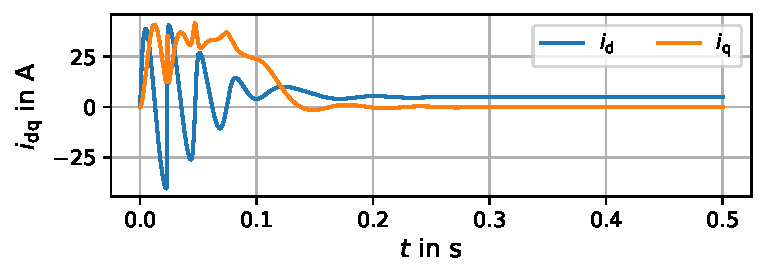
\includegraphics{ex05/i_dq_noLoad.pdf}
        \caption{Transient process of an IM in the dq coordinate system.}
        \label{fig:i_dq_noLoad}
    \end{solutionfigure}

    In \autoref{fig:i_ab_noLoad} the current in the $\upalpha, \upbeta$ coordinate system is visualized. The transient process is also clearly visible in this coordinate system.
    \begin{solutionfigure}[h]
        \centering
        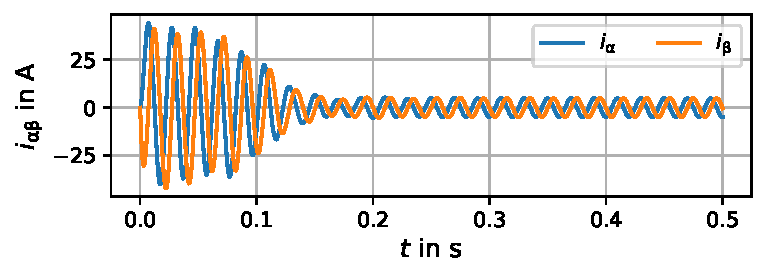
\includegraphics{ex05/i_alphaBeta_noLoad.pdf}
        \caption{Transient process of an IM in the $\upalpha \upbeta$ coordinate system.}
        \label{fig:i_ab_noLoad}
    \end{solutionfigure}

    \autoref{fig:i_abc_noLoad} shows the transient process of the current in the three-phase abc coordinate system.
    
    Compared to the abc current plot, one can observe also a sinusoidal signalform with the same amplitude and frequency evolution, while the phase difference between the currents is 120° in abc and 90° in $\upalpha\upbeta$. This fits to the expectations resulting from the amplitude-invariant Clarke transformation.
    \begin{solutionfigure}[h]
        \centering
        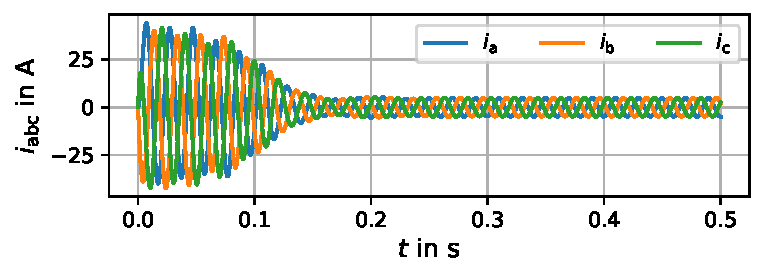
\includegraphics{ex05/i_abc_noLoad.pdf}
        \caption{Transient process of an IM in the abc coordinate system.}
        \label{fig:i_abc_noLoad}
    \end{solutionfigure}

    The electrical angular frequency of the stator and the angular frequency of the rotor are shown in \autoref{fig:speed_noLoad}. Due to the no load operation (also no friction) of the IM, the angular frequency of the rotor is equal to the angular electrical stator frequency.
    \begin{solutionfigure}[h]
        \centering
        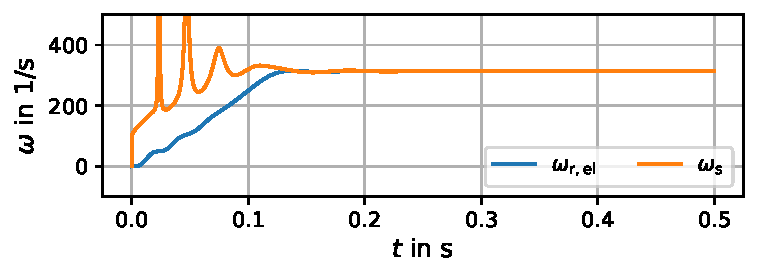
\includegraphics{ex05/speed_noLoad.pdf}
        \caption{Electric angular frequency of the stator and angular frequency of the rotor during the transient process at no load.}
        \label{fig:speed_noLoad}
    \end{solutionfigure}

    The produced torque is shown in \autoref{fig:torque_noLoad}. During the transient process, very high torque values are reached and an oscillation of the rotor is visible. In the steady state, the torque is equal to zero, due to the no-load operation.
    \begin{solutionfigure}[h]
        \centering
        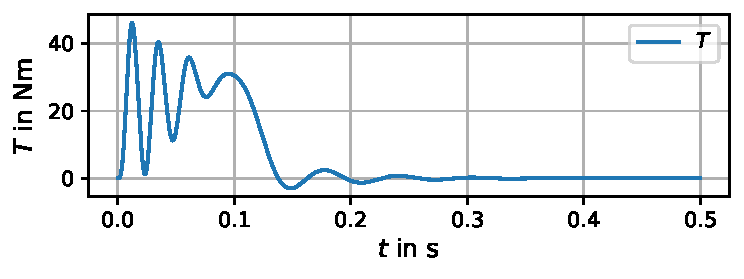
\includegraphics{ex05/torque_noLoad.pdf}
        \caption{Produced torque of an IM during the transient process at no load.}
        \label{fig:torque_noLoad}
    \end{solutionfigure}

    In \autoref{fig:rotorFlux_noLoad} the rotor flux is shown, which also shows the transient process. The d-axis of the coordinate system is oriented on the rotor flux and, therefore, the flux aligned to the q-axis is zero. Thus, only the rotor flux aligned to the d-axis is visualized.
    \begin{solutionfigure}[h]
        \centering
        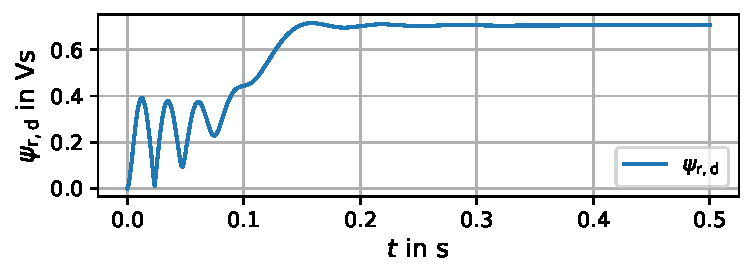
\includegraphics{ex05/psi_rd_noLoad.pdf}
        \caption{Rotor flux in dq coordinate system during the transient process at no load.}
        \label{fig:rotorFlux_noLoad}
    \end{solutionfigure}

    \begin{solutionfigure}[h]
        \centering
        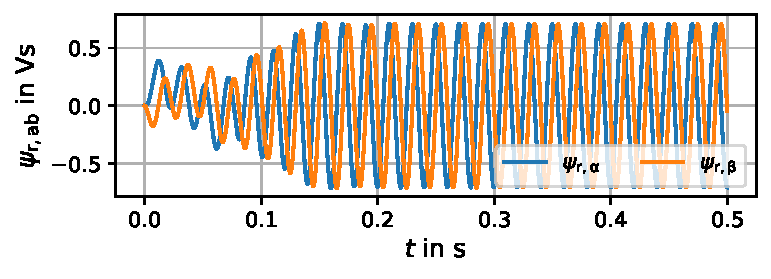
\includegraphics{ex05/psi_r_ab_noLoad.pdf}
        \caption{Rotor flux in $\upalpha\upbeta$ coordinate system during the transient process at no load.}
        \label{fig:rotorFlux_r_ab_noLoad}
    \end{solutionfigure}

    \begin{solutionfigure}[h]
        \centering
        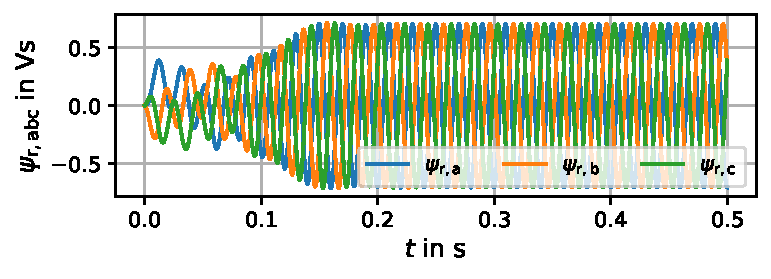
\includegraphics{ex05/psi_r_abc_noLoad.pdf}
        \caption{Rotor flux in abc coordinate system during the transient process at no load.}
        \label{fig:rotorFlux_r_abc_noLoad}
    \end{solutionfigure}

\end{solutionblock}


\FloatBarrier

%%%%%%%%%%%%%%%%%%%%%%%%%%%%%%%%%%%%%%%%%%%%%%%%%%%%%%%%%%%%%
\subtask{Add a speed dependent load with the following equation $T_{\mathrm{l}} = 0.00004*\omega_{\mathrm{r,el}}^2$ to the machine model. Repeat the simulation from the previous task. How does the currents, torque and flux change? In addition, how changes the rotational speed of the machine between these two operating points?}

\begin{solutionblock}
    In \autoref{fig:speed_friction} the speed of the stator and rotor field is visualized. For this simulation a load term representing the friction is added, thus this load is speed dependent. Hence, this results in a different speed of the rotor in the steady state in comparison to the stator field. This occurs due to the load of the machine, and is representing with the slip of the machine.
    \begin{solutionfigure}[h]
        \centering
        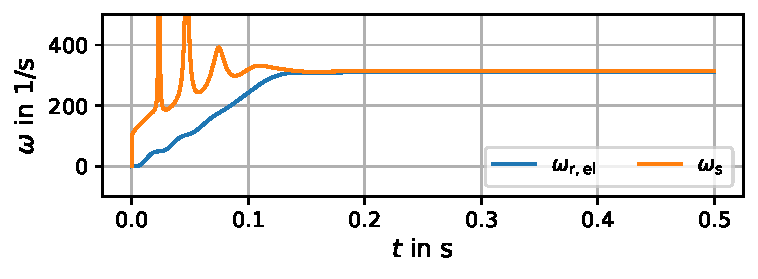
\includegraphics{ex05/speed_friction.pdf}
        \caption{Electrical angular frequency of the stator and angular frequency of the rotor during the transient process with a speed dependent load.}
        \label{fig:speed_friction}
    \end{solutionfigure}
    
    To highlight the difference between the stator and rotor field, in \autoref{fig:speed_zoom_friction} the boundaries of the vertical axis are limited. Hence, the speed difference in the steady state is clearly visible.
    \begin{solutionfigure}[h]
        \centering
        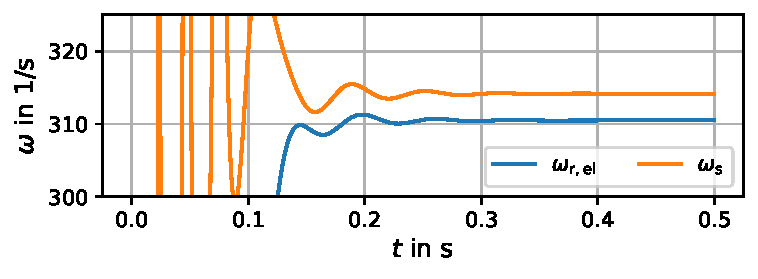
\includegraphics{ex05/speed_zoom_friction.pdf}
        \caption{Zoom into the electrical angular frequency of the stator and angular frequency of the rotor to visualize the difference in the steady state.}
        \label{fig:speed_zoom_friction}
    \end{solutionfigure}

    The produced torque during the transient process is shown in \autoref{fig:torque_friction}.
    \begin{solutionfigure}[h]
        \centering
        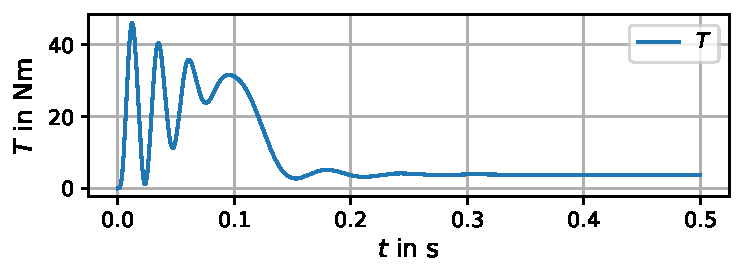
\includegraphics{ex05/torque_friction.pdf}
        \caption{Produced torque of an IM during the transient process and in the steady-state operation with a speed-dependent load.}
        \label{fig:torque_friction}
    \end{solutionfigure}
    \autoref{fig:torque_zoom_friction} shows a zoomed version of the produced torque to highlight the torque in the steady state.
    \begin{solutionfigure}[h]
        \centering
        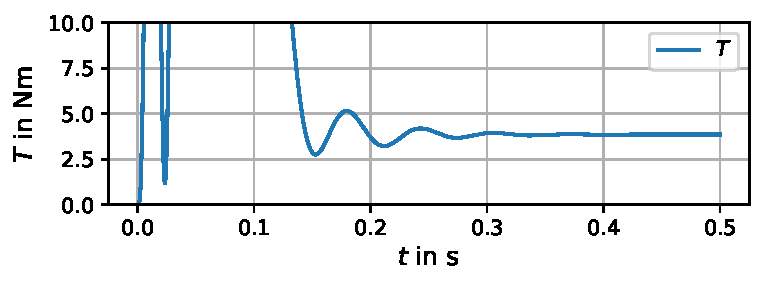
\includegraphics{ex05/torque_zoom_friction.pdf}
        \caption{Produced torque of an IM during the transient process and in the steady-state operation with a speed-dependent load.}
        \label{fig:torque_zoom_friction}
    \end{solutionfigure}

    In \autoref{fig:i_dq_friction} the currents in the dq coordinate system are visualized. Due to the load and, thus, the generated torque, the current $i_{\mathrm{q}}$ is no longer zero in the steady state. 
    \begin{solutionfigure}[h]
        \centering
        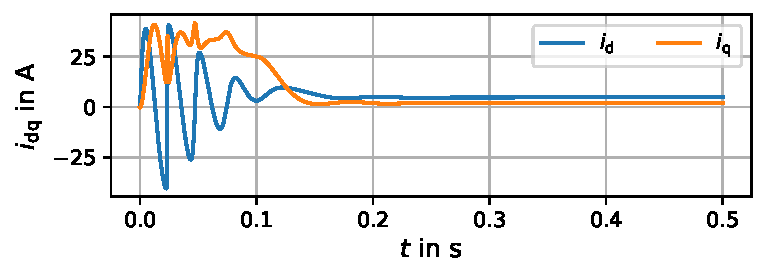
\includegraphics{ex05/i_dq_friction.pdf}
        \caption{Currents in dq coordinate system of an IM during the transient process and in the steady-state operation with a speed-dependent load.}
        \label{fig:i_dq_friction}
    \end{solutionfigure}

    \begin{solutionfigure}[h]
        \centering
        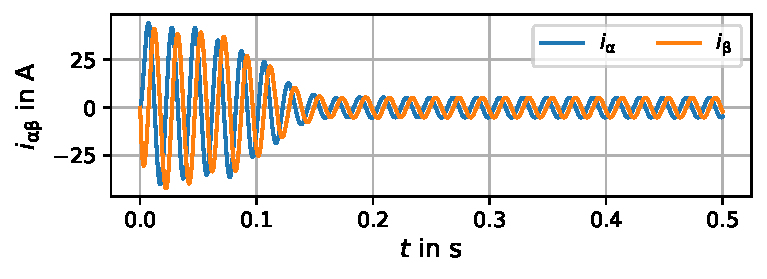
\includegraphics{ex05/i_alphaBeta_friction.pdf}
        \caption{Currents in $\upalpha \upbeta$ coordinate system of an IM during the transient process and in the steady-state operation with a speed-dependent load.}
        \label{fig:i_ab_friction}
    \end{solutionfigure}

    \begin{solutionfigure}[h]
        \centering
        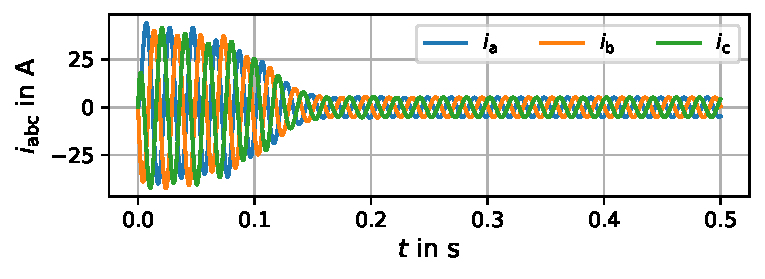
\includegraphics{ex05/i_abc_friction.pdf}
        \caption{Currents in abc coordinate system of an IM during the transient process and in the steady-state operation with a speed-dependent load.}
        \label{fig:i_abc_friction}
    \end{solutionfigure}

    \begin{solutionfigure}[h]
        \centering
        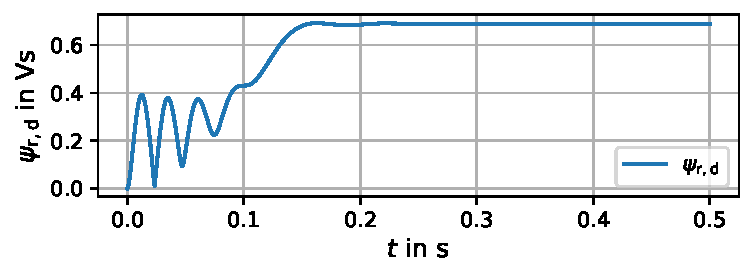
\includegraphics{ex05/psi_rd_friction.pdf}
        \caption{Rotor flux linkage in dq coordinate system of an IM during the transient process and in the steady-state operation with a speed-dependent load.}
        \label{fig:psi_rq_friction}
    \end{solutionfigure}

    \begin{solutionfigure}[h]
        \centering
        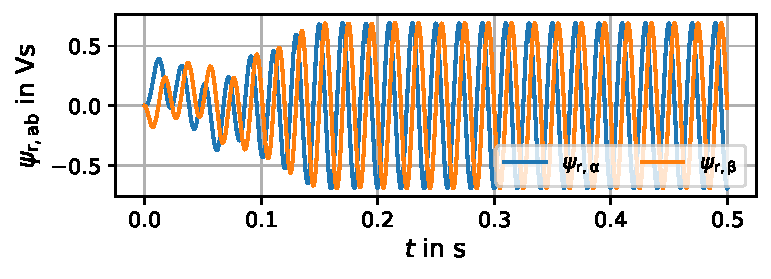
\includegraphics{ex05/psi_r_ab_friction.pdf}
        \caption{Rotor flux linkage in $\upalpha\upbeta$ coordinate system of an IM during the transient process and in the steady-state operation with a speed-dependent load.}
        \label{fig:psi_r_ab_friction}
    \end{solutionfigure}

    \begin{solutionfigure}[h]
        \centering
        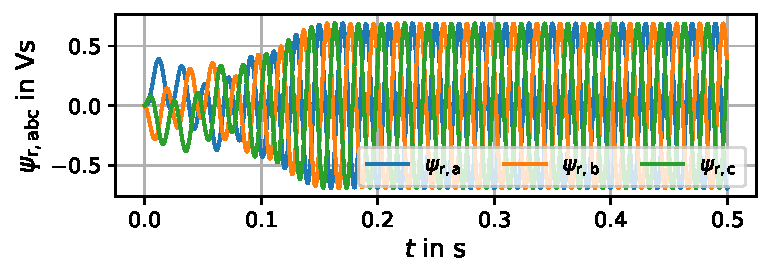
\includegraphics{ex05/psi_r_abc_friction.pdf}
        \caption{Rotor flux linkage in abc coordinate system of an IM during the transient process and in the steady-state operation with a speed-dependent load.}
        \label{fig:psi_r_abc_friction}
    \end{solutionfigure}



\end{solutionblock}


\FloatBarrier

%%%%%%%%%%%%%%%%%%%%%%%%%%%%%%%%%%%%%%%%%%%%%%%%%%%%%%%%%%%%%
%% Task 2 %%
%%%%%%%%%%%%%%%%%%%%%%%%%%%%%%%%%%%%%%%%%%%%%%%%%%%%%%%%%%%%%

\task{Steady-state operation of an induction machine}

An induction machine with the characteristics in Tab.~\ref{tab:characteristicsIM_task2} is given.
\begin{table}[htb]
    \caption{Characteristics of the given induction machine.}
    \centering
    \begin{tabular}{lll}\toprule
    Symbol  & Description       & Values \\
    \midrule
    $U_{\mathrm{n}}$    & Nominal voltage           & $\SI{380}{\volt}$ \\
    $I_{\mathrm{n}}$    & Nominal phase current     & $\SI{54}{\ampere}$ \\
    $f_{\mathrm{s,n}}$  & Nominal frequency         & $\SI{50}{\hertz}$ \\
    $P_{\mathrm{n}}$    & Nominal power             & $\SI{25}{\kilo\watt}$ \\
    $n_{\mathrm{n}}$    & Nominal speed             & $\SI{1465}{\per\minute}$ \\
    $\cos(\varphi)$     & Power factor              & 0.77 \\
    \midrule
    $R_{\mathrm{s}}$    & Stator resistance         & $\SI{0.48}{\Omega}$ \\
    $R_{\mathrm{r}}'$    & Rotor resistance          & $\SI{85}{\milli\Omega}$ \\
    $M$                 & Mutual inductance         & $\SI{100}{\milli\henry}$ \\
    $L_{\mathrm{\sigma,s}}$    & Stator leakage inductance  & $\SI{2}{\milli\henry}$ \\
    $L_{\mathrm{\sigma,r}}'$    & Rotor leakage inductance   & $\SI{2}{\milli\henry}$ \\
    \bottomrule
    \end{tabular}
    \label{tab:characteristicsIM_task2}
\end{table}


%%%%%%%%%%%%%%%%%%%%%%%%%%%%%%%%%%%%%%%%%%%%%%%%%%%%%%%%%%%%%
\subtask{Determine the amplitude of the complex AC voltage $\hat{U}$ and current phasor $\hat{I}$.}

\begin{solutionblock}
    The amplitude of the line-to-line voltage is given with
    \begin{equation}
    \hat{U} = \sqrt{2}\cdot \SI{380}{\volt}
    = \SI{537.4}{\volt},
    \end{equation}
    and, therefore, the amplitude of the phase-to-star-point voltage is defined as:
    \begin{equation}
    \hat{U}_{\mathrm{star}} = \frac{\SI{380}{\volt}}{\sqrt{3}}\cdot \sqrt{2} = \SI{310.9}{\volt}.
    \end{equation}

    Furthermore, the current amplitude is defined by:
    \begin{equation}
        \hat{I} = \sqrt{2} I = \sqrt{2} \cdot \SI{54}{\ampere} = \SI{76.4}{\ampere}.
    \end{equation}
\end{solutionblock}

%%%%%%%%%%%%%%%%%%%%%%%%%%%%%%%%%%%%%%%%%%%%%%%%%%%%%%%%%%%%%
\subtask{Determine the number of pole pairs $p$.}

\begin{solutionblock}
    The stator frequency is given with $f_{\mathrm{s}}$ = 50 Hz, which leads to the synchronous rotational speed of the electrical frequency as follows:
    \begin{equation}
        n_{\mathrm{syn,el}} = \SI{50}{\hertz} \cdot \SI{60}{\second\per\minute}
        = \SI{3000}{\per\minute}.
    \end{equation}
    
    The nominal speed is given with $n_{\mathrm{n}} = \SI{1465}{\per\minute}$, which is associated with a synchronous speed of $n_{\mathrm{syn,mech}} = \SI{1500}{\per\minute}$.
    
    Therefore, the number of pole pairs is defined with:
    \begin{equation}
        p = \frac{n_{\mathrm{syn,el}}}{n_{\mathrm{syn,mech}}}
        = \frac{\SI{3000}{\per\minute}}{\SI{1500}{\per\minute}}
        = 2.
    \end{equation}

\end{solutionblock}

%%%%%%%%%%%%%%%%%%%%%%%%%%%%%%%%%%%%%%%%%%%%%%%%%%%%%%%%%%%%%
\subtask{Calculate the rated slip $s_{\mathrm{n}}$. Which slip occurs at an ideal no-load operation (no firction)?}

\begin{solutionblock}
    The slip is calculated by:
    \begin{equation}
        s_{\mathrm{n}} = \frac{\omega_{\mathrm{slip,n}}}{\omega_{\mathrm{s}}}
        = \frac{\omega_{\mathrm{s}}-p \omega_{\mathrm{r}}}{\omega_{\mathrm{s}}}
        = \frac{\SI{2\pi\cdot \frac{3000}{60}}{\per\second}- 2 \cdot \SI{2\pi \cdot \frac{1465}{60}}{\per\second}}{\SI{2\pi \cdot \frac{3000}{60}}{\per\second}}
        = 0.023,
    \end{equation}
    where $\omega_{\mathrm{r}}$ is the rotor speed.
    At an ideal no-load operation (also no friction), the rotor has the same speed as the stator field and, therefore, $s$ = 0.
\end{solutionblock}

%%%%%%%%%%%%%%%%%%%%%%%%%%%%%%%%%%%%%%%%%%%%%%%%%%%%%%%%%%%%%
\subtask{Calculate the apparent, the reactive and the electrical power. In addition, determine the efficiency $\eta_{\mathrm{n}}$ for the rated operating point.}

\begin{solutionblock}
    The apparent power is calculated with
    \begin{equation}
        S = \sqrt{3} U I
        = \sqrt{3} \cdot \SI{380}{\volt} \cdot \SI{54}{\ampere}
        = \SI{35.541}{\kilo\volt\ampere},
    \end{equation}
    
    and, the electrical power is determined with the power factor in the task as follows:
    \begin{equation}
        P_{\mathrm{el,n}} = \sqrt{3} U I \cos(\varphi)
        = \sqrt{3} \cdot \SI{380}{\volt} \cdot \SI{54}{\ampere} \cdot 0.77
        = \SI{27.367}{\kilo\watt}.
    \end{equation}

    The angle of the phase shift is calculated by:
    \begin{equation}
        \varphi = \cos^{-1}(0.77) = \SI{39.6}{\degree}.
    \end{equation}

    Hence, the reactive power yields:
    \begin{equation}
        Q = \sqrt{3} U I \sin(\varphi)
        = \sqrt{3} \cdot \SI{380}{\volt} \cdot \SI{54}{\ampere} \cdot \sin(\SI{39.6}{\degree})
        = \SI{22.655}{\kilo\volt\ampere}.
    \end{equation}


    The efficiency results as:
    \begin{equation}
        \eta_{\mathrm{n}} = \frac{P_{\mathrm{mech,n}}}{P_{\mathrm{el,n}}} = \frac{\SI{25}{\kilo\watt}}{\SI{27.367}{\kilo\watt}}
        = 0.914.
    \end{equation}
\end{solutionblock}

%%%%%%%%%%%%%%%%%%%%%%%%%%%%%%%%%%%%%%%%%%%%%%%%%%%%%%%%%%%%%
\subtask{Determine the nominal torque generated by the induction machine.}

\begin{solutionblock}
    The torque is calculated as:
    \begin{equation}
        T_{\mathrm{n}} = \frac{P_{\mathrm{mech}}}{\omega_{\mathrm{mech}}}
        = \frac{\SI{25}{\kilo\watt}}{\SI{2\pi\cdot \frac{1465}{60}}{\per \second}}
        = \SI{163}{\newton \metre}.
    \end{equation}
\end{solutionblock}

%%%%%%%%%%%%%%%%%%%%%%%%%%%%%%%%%%%%%%%%%%%%%%%%%%%%%%%%%%%%%
\subtask{Calculate the starting $T_{\mathrm{0}}$ and the maximum torque $T_{\mathrm{max}}$. For the latter determine first the slip $s_{\mathrm{max}}$ at the operating point with the maximum torque.}

\begin{solutionblock}
    The slip at the maximum torque operating point is defined by
    \begin{equation}
        s_{\mathrm{max}} = \frac{R_{\mathrm{r}}'}{\sigma \left(L_{\mathrm{\sigma,r}}' + M\right) \omega_{\mathrm{s}}}
        = \frac{\SI{85}{\milli\Omega}}{0.038 \cdot (\SI{2}{\milli\henry}+\SI{100}{\milli\henry}) \cdot \SI{2\pi\cdot 50}{\per\second}}
        = 0.068,
    \end{equation}
    with the leakage coefficient:
    \begin{align}
        \begin{split}
            \sigma &= 1- \frac{M^2}{(M+L_{\mathrm{\sigma,s}})(M+L_{\mathrm{\sigma,r}}')}\\
            &= 1 - \frac{\left(\SI{100}{\milli\henry}\right)^2}{\left(\SI{102}{\milli\henry}\right)\cdot\left(\SI{102}{\milli\henry}\right)}\\
            &= 0.038.
        \end{split}
    \end{align}

    Hence, the maximum torque is calculated with:
    \begin{align}
        \begin{split}
            T_{\mathrm{max}} &= \frac{3}{2}p \frac{U_{\mathrm{s}}^2}{\omega_{\mathrm{s}}^2}\frac{M^2}{\sigma \left(L_{\mathrm{\sigma,s}}+M \right)^2\left(L_{\mathrm{\sigma,r}}'+M\right)} \\
            &= \frac{3}{2}\cdot2\cdot\frac{\frac{\SI{380}{\volt}}{\sqrt{3}}}{\left(\SI{2\pi\cdot 50}{\per\second}\right)^2} \cdot \frac{\SI{100}{\milli\henry}}{0.038\cdot\left(\SI{102}{\milli\henry}\right)^2 \cdot \left(\SI{102}{\milli\henry}\right)}\\
            &= \SI{355}{\newton\metre}.
        \end{split}
    \end{align}

    The starting torque is determined as follows:
    \begin{equation}
        T_{\mathrm{0}} = T_{\mathrm{max}} \frac{2 s_{\mathrm{max}}}{1 + s_{\mathrm{max}}^2}
        = \SI{355}{\newton\metre}\cdot \frac{2 \cdot 0.068}{1 + 0.068^2} = \SI{48.3}{\newton\metre}.
    \end{equation}
\end{solutionblock}


%%%%%%%%%%%%%%%%%%%%%%%%%%%%%%%%%%%%%%%%%%%%%%%%%%%%%%%%%%%%%
\subtask{Determine the stator currents $I_{\mathrm{s,dq}}$, and, in addition, the induced rotor currents $I_{\mathrm{r,dq}}$.}

\begin{solutionblock}
    Derived from the lecture notes, the stator currents are calculated as follows:
    \begin{align}
        \begin{split}
        I_{\mathrm{s,d}} &= \frac{U_{\mathrm{s}}}{\omega_{\mathrm{s}}} \frac{\sigma^2\omega_{\mathrm{slip}}^2 \left(L_{\mathrm{\sigma,s}}+M\right)\left(L_{\mathrm{\sigma,r}}'+M\right)^3 + \left(L_{\mathrm{\sigma,r}}'+M\right)\left(L_{\mathrm{\sigma,s}}+M\right)\left(R_{\mathrm{r}}'\right)^2 - M^2 \left(R_{\mathrm{r}}'\right)^2}{\sigma \left(L_{\mathrm{\sigma,s}}+M\right)^2 \left(L_{\mathrm{\sigma,r}}'+M\right)\omega_{\mathrm{slip}}\left(\sigma^2 \omega_{\mathrm{slip}}^2 \left(L_{\mathrm{\sigma,r}}'+M\right)^2 + \left(R_{\mathrm{r}}'\right)^2\right)}\\
        &= \SI{3.3}{\ampere},
        \end{split}
    \end{align}
    
    \begin{equation}
        I_{\mathrm{s,d}} = \frac{U_{\mathrm{s}}}{\omega_{\mathrm{s}}} \frac{M^2}{\sigma\left(L_{\mathrm{\sigma,s}}+M\right)^2 \left(L_{\mathrm{\sigma,r}}'+M\right)} \frac{1}{\frac{\omega_{\mathrm{slip}}}{\omega_{\mathrm{max}}} + \frac{\omega_{\mathrm{max}}}{\omega_{\mathrm{slip}}}}
        = \SI{51.8}{\ampere}.
    \end{equation}
    
    
    The rotor currents are calculated as follows:
    \begin{equation}
        I_{\mathrm{r,d}} = -U_{\mathrm{s}} \frac{M s}{\left(L_{\mathrm{\sigma,s}}+M\right) R_{\mathrm{r}}'}\frac{1}{\frac{\omega_{\mathrm{slip}}}{\omega_{\mathrm{max}}} + \frac{\omega_{\mathrm{max}}}{\omega_{\mathrm{slip}}}}
        = \SI{-18.06}{\ampere},
    \end{equation}

    \begin{equation}
        I_{\mathrm{r,q}} = -\frac{U_{\mathrm{s}}}{\omega_{\mathrm{s}}}\frac{M}{\sigma \left(L_{\mathrm{\sigma,s}}+M\right)\left(L_{\mathrm{\sigma,r}}'+M\right)}\frac{1}{\frac{\omega_{\mathrm{slip}}}{\omega_{\mathrm{max}}} + \frac{\omega_{\mathrm{max}}}{\omega_{\mathrm{slip}}}}
        = \SI{-52.9}{\ampere}.
    \end{equation}

    

\end{solutionblock}


%%%%%%%%%%%%%%%%%%%%%%%%%%%%%%%%%%%%%%%%%%%%%%%%%%%%%%%%%%%%%
\subtask{Calculate the losses in the stator winding and in the rotor.}

\begin{solutionblock}
    The stator current is determined by
    \begin{equation}
        I_{\mathrm{s,dq}} = \sqrt{I_{\mathrm{s,d}}^2 + I_{\mathrm{s,q}}^2}
        = \sqrt{\left(\SI{3.3}{\ampere}\right)^2 + \left(\SI{51.8}{\ampere}\right)^2}
        = \SI{51.9}{\ampere},
    \end{equation}
    which results to the stator winding losses as follows:
    \begin{equation}
        P_{\mathrm{l,stator}} = \frac{3}{2} I_{\mathrm{s,dq}}^2 R_{\mathrm{s}}
        = \frac{3}{2} \cdot \left(\SI{51.9}{\ampere} \right)^2 \cdot \SI{0.48}{\Omega}
        = \SI{1939.4}{\watt}.
    \end{equation}

    The rotor current is calculated in the same way. This leads to
    \begin{equation}
        I_{\mathrm{r,dq}} = \sqrt{I_{\mathrm{r,d}}^2 + I_{\mathrm{r,q}}^2}
        = \sqrt{\left(\SI{-18.1}{\ampere}\right)^2 + \left(\SI{-52.9}{\ampere}\right)^2}
        = \SI{55.9}{\ampere},
    \end{equation}
    and the ohmic rotor losses are calculated with:
    \begin{equation}
        P_{\mathrm{l,rotor}} = \frac{3}{2} I_{\mathrm{r,dq}}^2 R_{\mathrm{r}}'
        = \frac{3}{2} \cdot \left(\SI{55.9}{\ampere} \right)^2 \cdot \SI{85}{\milli\Omega}
        = \SI{398.4}{\watt}.
    \end{equation} 


\end{solutionblock}


%%%%%%%%%%%%%%%%%%%%%%%%%%%%%%%%%%%%%%%%%%%%%%%%%%%%%%%%%%%%%
\subtask{Draw the space vector diagram for the operation under rated conditions including the vectors $\underline{u}_{\mathrm{s}}$, $\underline{i}_{\mathrm{s}}$, $\underline{\psi}_{\mathrm{s}}$ and $\frac{\mathrm{d}}{\mathrm{d}t} \underline{\psi}_{\mathrm{s}}$. Assume that the current vector $\underline{i}_{\mathrm{s}}$ is oriented along the x-axis of the Cartesian coordinate system.}

\begin{solutionblock}
    The current is aligned with the x-axis of the Cartesian coordinate system. Therefore, the current is given with:
    \begin{equation}
        \underline{i}_{\mathrm{s}} = \sqrt{2} I e^{\mathrm{j}0^{\circ}}
        = \SI{76.37}{\ampere} \cdot e^{\mathrm{j}0^{\circ}}.
    \end{equation}

    The angle shift between the voltage and current is calculated by
    \begin{equation}
        \varphi_{\mathrm{ui}} = \SI{39.65}{\degree},
    \end{equation}

    therefore, the voltage is defined as follows:
    \begin{equation}
        \underline{u}_{\mathrm{s}} = \sqrt{2} U e^{\mathrm{j} \varphi_{\mathrm{ui}}}
        = \SI{310.27}{\volt} \cdot e^{\mathrm{j}39.65^{\circ}}
        = \SI{238.89}{\volt} + \mathrm{j} \SI{197.98}{\volt}.
    \end{equation}

    The stator resistance $R_{\mathrm{s}}$ is given in the task. Hence, the voltage equation is defined as:
    \begin{equation}
        \underline{u}_{\mathrm{s}} = R_{\mathrm{s}} \underline{i}_{\mathrm{s}} + \frac{\mathrm{d}}{\mathrm{d}t}\psi_{\mathrm{s}}.
    \end{equation}

    Rearranging leads to:
    \begin{align}
        \begin{split}
        \frac{\mathrm{d}}{\mathrm{d}t}\psi_{\mathrm{s}} &= \underline{u}_{\mathrm{s}} - R_{\mathrm{s}} \underline{i}_{\mathrm{s}} \\
        &= \SI{238.89}{\volt} + \mathrm{j} \SI{197.98}{\volt} - \SI{0.48}{\Omega} \cdot \SI{76.37}{\ampere} \\
        &= \SI{202.23}{\volt} + \mathrm{j} \SI{197.98}{\volt} \\
        &= \SI{283}{\volt} \cdot e^{\mathrm{j}44.4^{\circ}}.
        \end{split}
    \end{align}

    The stator flux vector is defined as
    \begin{equation}
        \underline{\psi}_{\mathrm{s}}(t) = \psi_{\mathrm{s}}(t) \cdot e^{\mathrm{j}\varphi_{\mathrm{s}}(t)},
    \end{equation}

    and the differentiation (under consideration of the product rule) results in:
    \begin{equation}
        \frac{\mathrm{d}}{\mathrm{d}t}\underline{\psi}_{\mathrm{s}}(t)
        = \frac{\mathrm{d}}{\mathrm{d}t} \psi_{\mathrm{s}}(t) \cdot e^{\mathrm{j}\varphi_{\mathrm{s}}(t)} + \mathrm{j} \omega_{\mathrm{\varphi_s}} \cdot \underline{\psi}_{\mathrm{s}}(t).
    \end{equation}

    Due to the steady state, the change of the flux amplitude $\left(\frac{\mathrm{d}}{\mathrm{d}t}\psi(t)\right)$ is zero. The flux vector rotates with the speed $\omega$, therefore, the flux vector is determined as follows:
    \begin{equation}
        \underline{\psi}_{\mathrm{s}}(t)
        = \frac{\SI{283}{\volt} \cdot e^{\mathrm{j}44.4^{\circ}}}{\SI{314.16}{\per\second}\cdot e^{\mathrm{j}90^{\circ}}}
        = \SI{0.90}{\volt\second} \cdot e^{-\mathrm{j}\SI{45.6}{\degree}}.
    \end{equation}


    \begin{solutionfigure}
        \centering
        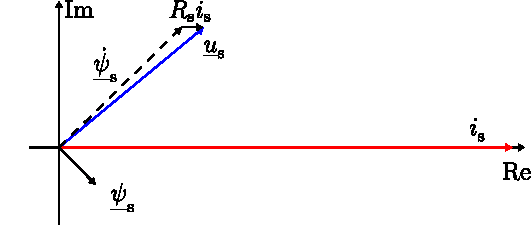
\includegraphics{ex05/vectorDiagram_IM.pdf}
        \caption{Resulting vector diagram of the induction machine in steady state. The scala for the voltage is 1 cm $\widehat{=}~\SI{100}{\volt} $, for the flux linkage 1 cm $\widehat{=}~\SI{1}{\volt\second}$ and for the current 1 cm $\widehat{=}~\SI{10}{\ampere}$.}
        \label{fig:vectorDiagram_IM}
    \end{solutionfigure}


\end{solutionblock}